Voici une présentation de l'interface et ses fonctionnalités.

\subsection{Interface}
Voici comment se présente notre interface : 
\begin{figure}[!h]
    \centering
    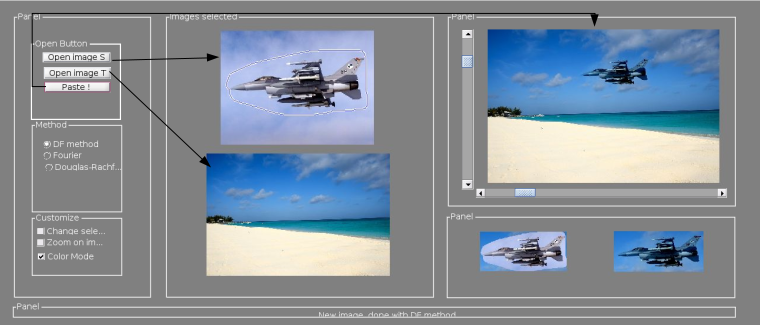
\includegraphics[scale = 0.5]{Images/interface.png}
    \caption{Interface 1.0}
\end{figure}{}
\subsubsection{Ouverture d'images}
Vous pouvez ouvrir n'importe quelle image en cliquant sur les boutons situés en haut à gauche de l'interface. En cliquant sur eux, une boite de dialogue vous proposera de choisir une image présente sur votre ordinateur. Une fois sélectionnée cette image sera affichée sur l'interface et vous pourrez travailler dessus. Image S correspond à l'image Source, c'est l'image que vous souhaitez coller. Et l'image T représente l'image Target, l'image d'arrière plan.\newline
\subsubsection{Sélection}
Une fois vos deux images ouvertes, il vous faut sélectionner la partie de l'image S (8) que vous souhaitez coller dans l'image T. Pour cela cliquez une première fois sur l'image S : celle du haut puis cliquez une seconde fois pour dessiner sur l'image, la partie que vous souhaitez extraire. 
\newline
Pour la seconde image, faites de même (9), cliquez une première fois sur l'image puis cliquez une seconde fois pour choisir l'endroit où vous souhaitez coller la partie sélectionnée plus tôt.  Voici ce que vous devriez obtenir. 
\subsubsection{Choix des méthodes}
Vous pouvez sélectionner la méthode avec laquelle vous voulez coller l'image S dans l'image T. Vous avez pour l'instant deux méthodes : 
\begin{itemize}
    \item Avec les différences finies (4)
    \item Avec Fourier (5)
\end{itemize}{}

\subsubsection{Différences finies}
Une fois la méthode DF choisie, il vous suffit de cliquer sur le bouton "Paste!"(3)  pour afficher le résultat.
\subsubsection{Options}
Nous avons ajouté des options comme l'option de zoom (6) qui permet de zoomer sur une image pour voir de plus près le collage de l'image. 
\paragraph{ Amélioration avec change selection}
Ainsi nous avons ajouté, l'option Change sélection qui re-dimensionne automatique la sélection afin de résoudre ce pb. 
\paragraph{Mode couleur}
En sélectionnant le mode couleur, (8) vous pourrez travailler sur des images en couleur. 

\subsubsection{Sliders}
Vous pouvez bouger les sliders présents à droite afin de déplacer la zone collée dans l'image de fond. La solution au problème est alors automatiquement recalculée en fonction de l'endroit où l'objet à collé. 

\subsection{Organisation du code}
Nous avons organisé le code sous forme de classes. Le projet contient 4 classes principales, la classe, Fourier, la classe DFinies, la classe Douglas et enfin la classe  Mask. Notre projet contient aussi deux fonctions, la fonctions copier/coller et la fonction du gradient conjugué.

%%%%%%%%%%%%%%%%%%%%%%%%%%%%%%%%%%%%%%%%%%%%%%%%%%%

\begin{figure}
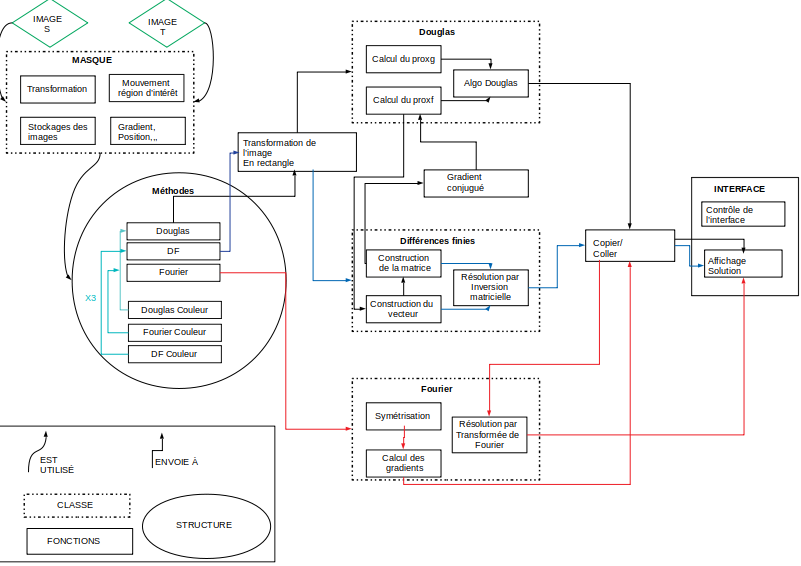
\includegraphics[scale=0.65]{Images/code/schema.png}
\caption{Structure et interactions du code}
\end{figure}
\newpage

\paragraph{Explication du schéma}
Le code est organisé en différentes classes (4).
\paragraph{Douglas}
Cet algorithme étant plutôt long (en terme de temps), nous ne travaillerons pas sur l'image entière mais sur le plus petit rectangle autour de la sélection.En d'autre terme nous collerons l'image S sur une sous-image de T, que nous réinsérerons par la suite au bon endroit dans T. Afin de résoudre le problème à l'aide de l'algorithme de Douglas, nous avons crée une classe du même nom.  A l'intérieur de celle-ci nous calculons les opérateurs proximaux nécessaires. Avec une particularité, l'opérateur proximal de la norme, nécessite la construction d'une matrice. Afin d'éviter les doublons nous utilisons donc la classe FDSystem, pour calculer cette matrice, et le vecteur associé. Puis nous inversons le système à l'aide de l'algorithme du gradient conjugué. 
\paragraph{Différences finies}
Pour résoudre le problème avec les différences finies, la classe DFSystem, nous permet de calculer la matrice A, le vecteur b et enfin d'inverser le système pour trouver la solution. De la même manière que pour Douglas, nous ne travaillons pas sur l'image entière mais sur une sous-image que nous recollons au bon endroit à la fin.
\paragraph{Fourier}
Dans la classe Fourier nous symétrisons les images, puis calculons les gradients de celles-ci. Les images représentant les gradients sont par la suite fusionnées avant d'être envoyé à la fonction de résolution de la classe Fourier. 
\paragraph{Mask}
La classe Mask, permet le traitement d'images et de masque, elle est mise à jour pendant tout le programme. C'est notamment elle qui permet le découpage d'image, la fusion de deux images, le redimensionnement des masques si besoin. 
\paragraph{La fonction gradient conjugué}
Elle permet de trouver la solution au système Ax=b de manière plus rapide qu'une inversion dans matlab.
\paragraph{La fonction copier coller} 
Elle écrase certains pixels d'une image par les pixels d'une autre.